\chapter{Fundamentos}
\label{chap:fundamentos}
En este capítulo se expondrán y analizarán brevemente los trabajos previos en la materia de perfilado automático de usuarios en base a texto, que se han tenido en cuenta para la elaboración de las soluciones escogidas.
%TODO arreglar citas
\section{Estado del arte}%o referencia o trabajo relacionado
\label{sec:estado_arte}
Desde los primeros años del inicio de las redes sociales, el interés por la extracción automática de características demográficas latentes de usuarios se vio patente en una serie de trabajos tempranos. En 2007, \cite{ap_argamon_07} demostró como el estilo de escritura y otros aspectos socio-lingüísticos observados en textos procedentes de blogs en idioma inglés se ven afectados por características demográficas como la edad y género de los autores de los mismos. En este otro trabajo del 2006 \cite{ap_argamon_06}, se obtuvieron buenos resultados en la clasificación de género y edad (precisión mayor al 75\% para ambos) usando para la combinación de características basadas en estilo y basadas en contenido, en un corpus compuesto por textos provenientes de blogs en inglés. También se  tiene registro de varios trabajos que tratan el tema a partir de la creación de corpus en otros idiomas como \cite{profiling_urdu} en roman urdu.

Sin embargo, en los últimos años destacan especialmente, en materia de perfilado automático y \gls{author_analysis} en general, las competiciones organizadas por el PAN\footnote{\url{https://pan.webis.de/}}. Estas consisten en una serie de eventos científicos y tareas compartidas sobre texto digital forense y estilometría. Estas tareas se realizan anualmente y en la mayoría de ediciones se pueden encontrar tareas de perfilado de usuarios (\cite{pan:2014}, \cite{pan:2015}, \cite{pan:2016}).

%TODO maybe poner un cuadro con las ediciones del PAN y lo que se perfilaba género edad y en que idioma
Por otro lado, desde 2019 se empezaron a organizar la competición análoga al PAN en idioma español: el IberLEF\footnote{\url{http://sepln2023.sepln.org/iberlef/}}. Esta se enmarca dentro de la Sociedad Española para el Procesamiento del Lenguaje Natural (SEPLN) como una serie de tareas para promover la investigación de tareas de análisis, procesamiento y generación de textos en las lenguas ibéricas.

Sin embargo, a pesar de estas iniciativas recientes hay que tener en cuenta que los esfuerzos realizados en materia de perfilado automático de usuarios, están centrados mayoritariamente en el idioma inglés. Debido a la naturaleza multilingüe de muchos de los modelos y algoritmos, estos pueden ser adaptados a otros idiomas como el español sin demasiada dificultad. Sin embargo, otro tipo de recursos como pueden ser los conjuntos de entrenamiento para estos modelos son únicos para un idioma por lo tanto en este aspecto se nota en mayor medida la escasez con respecto al idioma inglés.

De este modo, pese al gran interés de este tipo de algoritmos en el idioma español el......
%TODO acabar
\section{Conjuntos de datos}
\label{sec:datasets}
Como nuestro objetivo consiste en conocer las características demográficas de los usuarios de la colección de \acrshort{blm} es necesario disponer de un corpus o conjunto de datos para entrenar los modelos perfilado automático.

%reducible/revisar--->
Lo ideal en este caso sería crear un corpus personalizado, a modo de conjunto de entrenamiento, lo más similar posible a la colección, es decir, preferiblemente a partir de textos del mismo foro de Reddit o de otro parecido al que se extrajo esta. Crear un corpus de un tamaño aceptable con estas características, supondría un proceso bastante difícil y costoso en tiempo, ya que la API de Reddit no permite obtener edad y género de manera sencilla.Sería necesario etiquetar manualmente las características demográficas de los usuarios: o bien preguntándoles directamente o bien realizando una labor de investigación sobre los mismos para averiguarlas.

%<----reducible/revisar
Por este motivo, se decidió usar un corpus con usuarios etiquetados ya creado. Existen varias opciones en idioma español en este sentido. En 2014, \cite{SpanText} crearon un corpus en español compuesto principalmente por texto formal (esto es con pocas palabras que no pertenecen al "diccionario", abreviaturas, vulgarismos...) a partir de texto extraídos de la web. No obstante, el lenguaje usado en la colección de \acrshort{blm} es más bien de tipo informal, es decir, contiene bastantes vulgarismos, extranjerismos 
 y expresiones de la jerga de las redes sociales. Por esta razón, fue que se descartó el corpus anterior en busca de otro procedente de redes sociales más informales como Reddit o Twitter. En este sentido, los conjuntos de datos creados por los organizadores de la tareas del PAN son las únicas opciones viables que se encontraron, que incluían ambos género y edad. Concretamente usaremos los particiones de los \gls{datasets} correspondientes a textos de Twitter en español de las competiciones de los años 2015\footnote{\url{https://zenodo.org/record/3745945}} y 2016\footnote{\url{https://zenodo.org/record/3745963}} (\cite{pan:2015} y \cite{pan:2016} respectivamente).
 
  \subsection{PAN author profiling 2015}
  \label{subsec:pan15}
 El conjunto de 2015, estaba compuesto por textos procedentes de Twitter completamente y estaba formado por una partición de entrenamiento y otra de test. Además de edad y género los autores de los texto de este \textit{dataset} estaban etiquetados con valores auto evaluados para los rasgos de personalidad, definidos mediante el Modelo de los 5 Grandes (\cite{5grandes}).

 En cuanto al formato de los \textit{datasets}, en el conjunto de 2015 cada autor aparece representado con un fichero .xml donde dentro del tag raíz author se encontraban situados los \textit{tweets}. Este contiene exactamente 100 \textit{tweets} distintos cada uno como contenido de un tag document hijo del tag raíz author. Por cada autor hay exactamente 100 tags.
 
 Para conocer las etiquetas de género, edad, y personalidad existe un único archivo en texto plano en el que aparece por cada autor una línea donde le se asocia sus valores demográficos y de personalidad. Como podemos ver en la figura \ref{fig:formato-dataset} el contenido del archivo está a modo de archivo .csv donde el separador es la cadena ":::". Las columnas del archivo se corresponderían con el indetificador del autor, rango de edad, género y valores de personlidad como se indica \cite{dataset:15}.
 \begin{figure}[hp!]
  \centering
    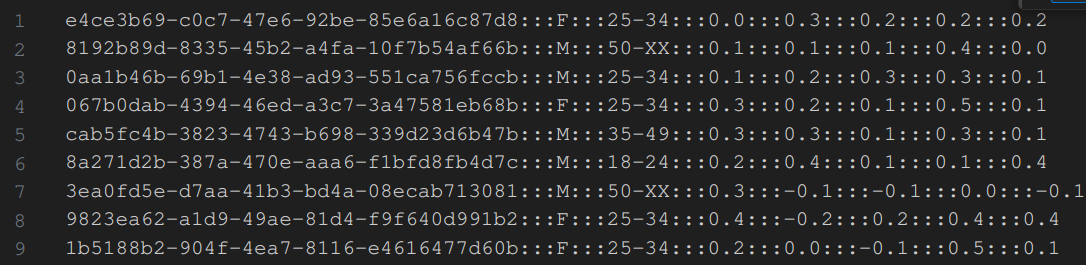
\includegraphics[width=\textwidth]{imaxes/formato_dataset.png}
  \caption{Formato archivo truth.txt \textit{dataset} 2015}
  \label{fig:formato-dataset}
\end{figure}

  \subsection{PAN author profiling 2016}
 Por otra parte, el conjunto de 2016 incluía una partición de entrenamiento formada por textos sacados de usuarios de Twitter y una partición de test formada por texto sacados de Blogs. Estos últimos utilizan un lenguaje más formal, habitualmente conteniendo poemas, canciones o fragmentos de texto no escritos por los usuarios etiquetados que podían afectar negativamente al rendimiento del algoritmo de perfilado. Por estas razones, se decidió utilizar únicamente la partición de entrenamiento para entrenar nuestro clasificador.
 
 El formato de este corpus es bastante similar al del 2015: cada autor aparece representado en un archivo .xml nombrado con un identificador único a partir del cual se puede sacar sus datos demográficos en un archivo truht.txt.
 
 La diferencia con el de 2015, está en que en vez de aparecer los tweets directamente en el .xml, aparecen las URLs a esos tweets. Además en vez haber exactamente 100 \textit{tweets} por autor, en la mayoría hay hasta 1000. Para conseguir los textos correspondientes a los \textit{tweets} el PAN disponía de un programa\footnote{\url{https://github.com/pan-webis-de/pan-code/tree/master/clef16/author-profiling/twitter-downloader}} que los descargaba y escribía directamente el texto de los mismos en los .xml. Sin embargo, desde 2020 la API de Twitter cambió y este programa dejó de funcionar\footnote{Enlace al issue de github donde lo indican: \url{https://github.com/pan-webis-de/pan-code/issues/3}}.
 
 Por este motivo, se decidió crear un web scraper que fuera leyendo las direcciones URL de los .xml que se correspondían con los tweets de los usuarios y descargara el texto de estos sin necesidad de usar la API de Twitter. Sin embargo, este proceso era mucho más lento que el uso del programa antes mencionado (1000 \textit{Tweets}/minuto frente a aproximadamente 30 \textit{Tweets}/minuto). Esto hizo que decidiera ejecutar de forma \textit{serveless} este programa diariamente en forma de notebook en Kaggle\footnote{\url{https://www.kaggle.com/}}, esta web permite programar ejecuciones de jupyter notebooks de forma asíncrona que pueden durar hasta 12 horas siendo 10 el número máximo de notebooks ejecutándose concurrentemente. De esta forma en un par de días ya tenía descargada toda la colección, sin contar los tweets y usuarios eliminados que eran bastantes. En la figura \ref{fig:scraper} se puede ver una captura de los logs resultantes de realizar una ejecución de 12 horas del \textit{scraper} para descargar los \textit{tweets} del \textit{dataset}.
 %En total hay 187995 tweets y 843.0269058295964 tweets por autor de media

 \noindent\begin{figure}[hp!]
  \centering
    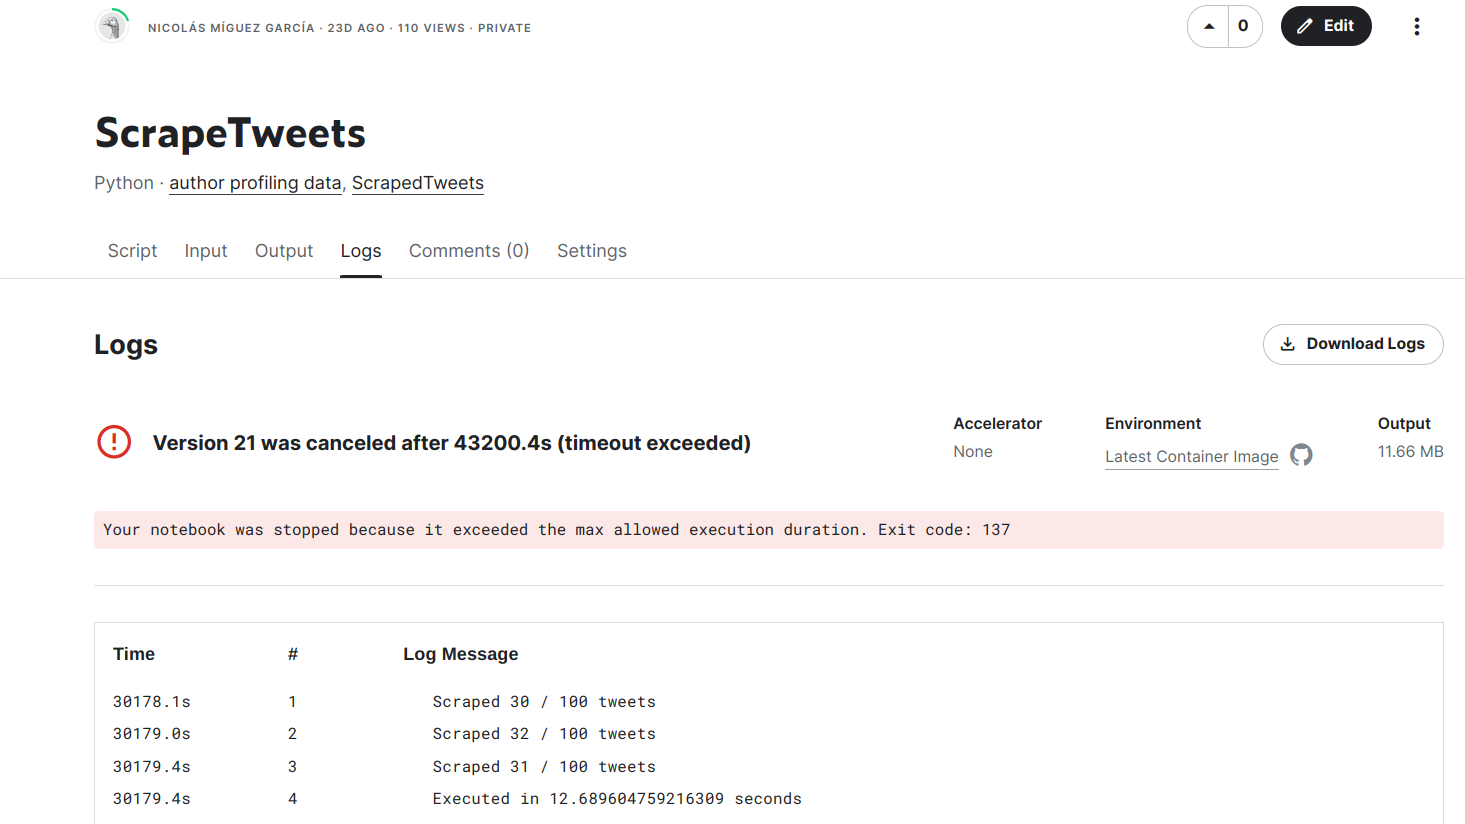
\includegraphics[width=\textwidth]{imaxes/scraper.png}
  \caption{Logs resultado de una ejecución del notebook a modo de \textit{scraper} para la obtención de los \textit{tweets} del \textit{dataset} de 2016}
  \label{fig:scraper}
\end{figure}
 
   \subsection{Distribución de usuarios de los \textit{dataset}}

   En la tabla \ref{tab:datasets_edad} podemos ver la distribución de autores en función de edad y género de ambos conjuntos. Como se puede observar los \textit{datasets} están equilibrados en cuestión de género, mientras que están bastante más desequilibrados en cuestión de edad.
   
   Vale la pena mencionar que aunque en el \textit{dataset} de 2016, originalmente había 250 de Training, al descargar los textos correspondientes a estos muchos de ellos no estaban disponibles (puesto que los \textit{tweets} eran se había publicado originalmente en el año 2013), pues se habían eliminado su cuenta de Twitter. Consecuentemente, descartando estos usuarios quedan un total de 222.
   \begin{table}[hp!]
    \centering
    \rowcolors{2}{white}{udcgray!25}
    \begin{tabular}{|l|ll|l|}
        \rowcolor{udcpink!25}
        \hhline{~|---}
        \multicolumn{1}{c|}{\cellcolor{white}} & \multicolumn{2}{c|}{\textbf{PAN-AP 2015}} & \textbf{PAN-AP 2016}\\ \hline
        Categoría & Training & Test & Training \\ \hline
        18-24 & 22 & 18 & 11\\
        25-34 & 46 & 44 & 54\\
        35-49 & 22 & 18 & 116\\
        +50 & 10 & 8 & 41\\ \hline
        Hombres & 50 & 44 & 111\\
        Mujeres & 50 & 44 & 111\\ \hline
        Total & 100 & 88 & 222\\ \hline  
    \end{tabular}%
    \caption{Distribución de usuarios en función de edad y género en los conjuntos de entrenamiento utilizados.}
    \label{tab:datasets_edad}
\end{table}

\section{Búsqueda y comparación de algoritmos}
En esta sección, se detalla la fase del proyecto consistente en 
 la investigación sobre los algoritmos o modelos existentes de clasificación de texto para tareas de perfilado automático de usuarios.
 
 El objetivo principal de esta fase era el análisis del estado del arte en este campo con la finalidad de escoger y replicar los algoritmos, de perfilado de usuario, más robustos para nuestro trabajo. En consecuencia, vale la pena resaltar que la intención no era realizar un modelo original desde cero sino utilizar uno ya implementado y del que se tenga conocimiento que reporta buenos resultados.
 
 Para ello, se orientó la búsqueda hacia las competiciones ya mencionadas en el apartado \ref{sec:estado_arte} como PAN (\cite{pan:2013}) o IberLef (\cite{iberlef2022}). Esto tiene dos motivos: primero que seleccionando los algoritmos de entre los participantes en una de estas competiciones, contamos con la información previa de la bondad de los algoritmos con los otros competidores, pudiendo así seleccionar los que mejor se comportaron en las mismas; por otra parte, estas competiciones al estar de alguna forma abiertas al público es más sencillo encontrar de forma pública las implementaciones de los algoritmos participantes en repositorios como Github\footnote{\url{https://github.com/}}.
 
En la tabla \ref{tab:comparacion-profilers} prueba se muestra una pequeña comparativa de los algoritmos del estado del arte con implementación disponible en Github. En ella se muestran en cada columna: la referencia a las \textit{working notes} del equipo participante de la tarea, la competición para la que se desarrolló, la posición final en la que quedó el equipo participante (teniendo en cuenta perfilado en idioma español solamente), el modelo de aprendizaje automático utilizado y un resumen muy general de las características extraídas para la clasificación del texto.

Como se puede ver en la tabla muchos de estos algoritmos usan modelos y características bastante similares entre ellos. En consecuencia, solo se decidieron replicar tres de ellos (\cite{loscalis22}, \cite{modaresi:2016} y \cite{grivas2015author}).


\begin{table}[hp!]
    \centering
    \rowcolors{2}{white}{udcgray!25}
    {
    \setlength{\tabcolsep}{0.4\tabcolsep}
        \begin{tabular}{|p{0.15\linewidth} |p{0.18\linewidth} |p{0.11\linewidth} |p{0.1\linewidth} | p{0.27\linewidth} |}
            \hline
            \rowcolor{udcpink!25}
            
            \textbf{Equipo} & \textbf{Competición}  & \textbf{Posición} & \textbf{Modelo} & \textbf{Características}\\ \hline
            Grivas \cite{grivas2015author} & PAN 2015 \cite{pan:2015} & 3º & \gls{svm} & Tfidf n-grams stylistic features\\
            Modaresi \cite{modaresi:2016} & PAN 2016 \cite{pan:2016} & 2º & \gls{lr} & Tfidf n-grams stylistic features\\
            Daneshvar \cite{Daneshvar2018} & PAN 2018 \cite{pan:2018} & 1º & \gls{svm} & Tfidf ngrams w LSA\\
            Bacciu \cite{bacciu2019bot} & PAN 2019 \cite{pan:2019} & 3º & \gls{svm} & Tfidf n-grams w LSA\\
            Baseline & PAN 2020 \cite{pan:2020} & & \gls{lr} & Tfidf n-grams\\
            LosCalis \cite{loscalis22} & IberLef 2022 \cite{iberlef2022} & 1º & \gls{mlp} & Embeddings (BERT + RoBERTa)\\
            Holgado \cite{holgado2022halbert} & IberLef 2022 \cite{iberlef2022} & 5º & \gls{em} & n-grams + embeddings + stylistic features\\ \hline
        \end{tabular}
    }
    \caption{Comparación de algoritmos del estado del arte en perfilado de usuarios de los cuales se encontró la implementación disponible en Github.}
    \label{tab:comparacion-profilers}
\end{table}

\subsection{Primera aproximación}
En primer lugar, tenemos al ganador de la competición del IberLef 2022: "PoliticEs 2022: Perfilado de usuarios para ideología política". Esta competición consistía en la predicción de género, profesión e ideología política binaria (izquierda y derecha) y multiclase (izquierda, centro-izquierda, centro-derecha y derecha) de usuarios de Twitter sobre un corpus de \textit{tweets} procedentes de periodistas, políticos y españoles.

En esta competición \cite{iberlef2022}, la mayoría de aproximaciones usadas por los participantes eran modelos basados en transformers \cite{vaswani2017attention}. Estos consistían en modelos de lenguaje pre-entrenados (BETO \cite{BETO}, MarIA \cite{MarIA}, BERT multilingüe, ALBERT...) afinados con el corpus de la competición, con el objetivo de extraer características del texto a nivel de documento. Este tipo de arquitecturas, basadas en transformers, son la gran novedad con respecto a los enfoques utilizados en competiciones de años anteriores del PAN. \\

%%%%%%%%%%%%%%%%%%%%%%%%%%%%%%%%%%%%%%%%%%%%%%%%%%%%%%%%%%%
% \subsubsection{Transformers y modelos de lenguaje}
% TODO 
% meter teoría sobre transformers y modelos de lenguaje
%%%%%%%%%%%%%%%%%%%%%%%%%%%%%%%%%%%%%%%%%%%%%%%%%%%%%%%%%%%

El enfoque utilizado por LosCalis \cite{loscalis22} por tanto, combinaba el modelo BERT \cite{devlin2019bert} pre-entrenado en idioma español, conocido como BETO \cite{BETO} junto con el modelo RoBERTa pre-entrenado en español, llamado MarIA \cite{MarIA}. Este emplea ambas arquitecturas para extracción de características a nivel de documento y en base a estas se entrena un perceptrón multicapa para decodificar las etiquetas de los usuarios. En la figura \ref{fig:arquitectura} se muestra la arquitectura del modelo utilizado.

\noindent\begin{figure}[hp!]
  \centering
    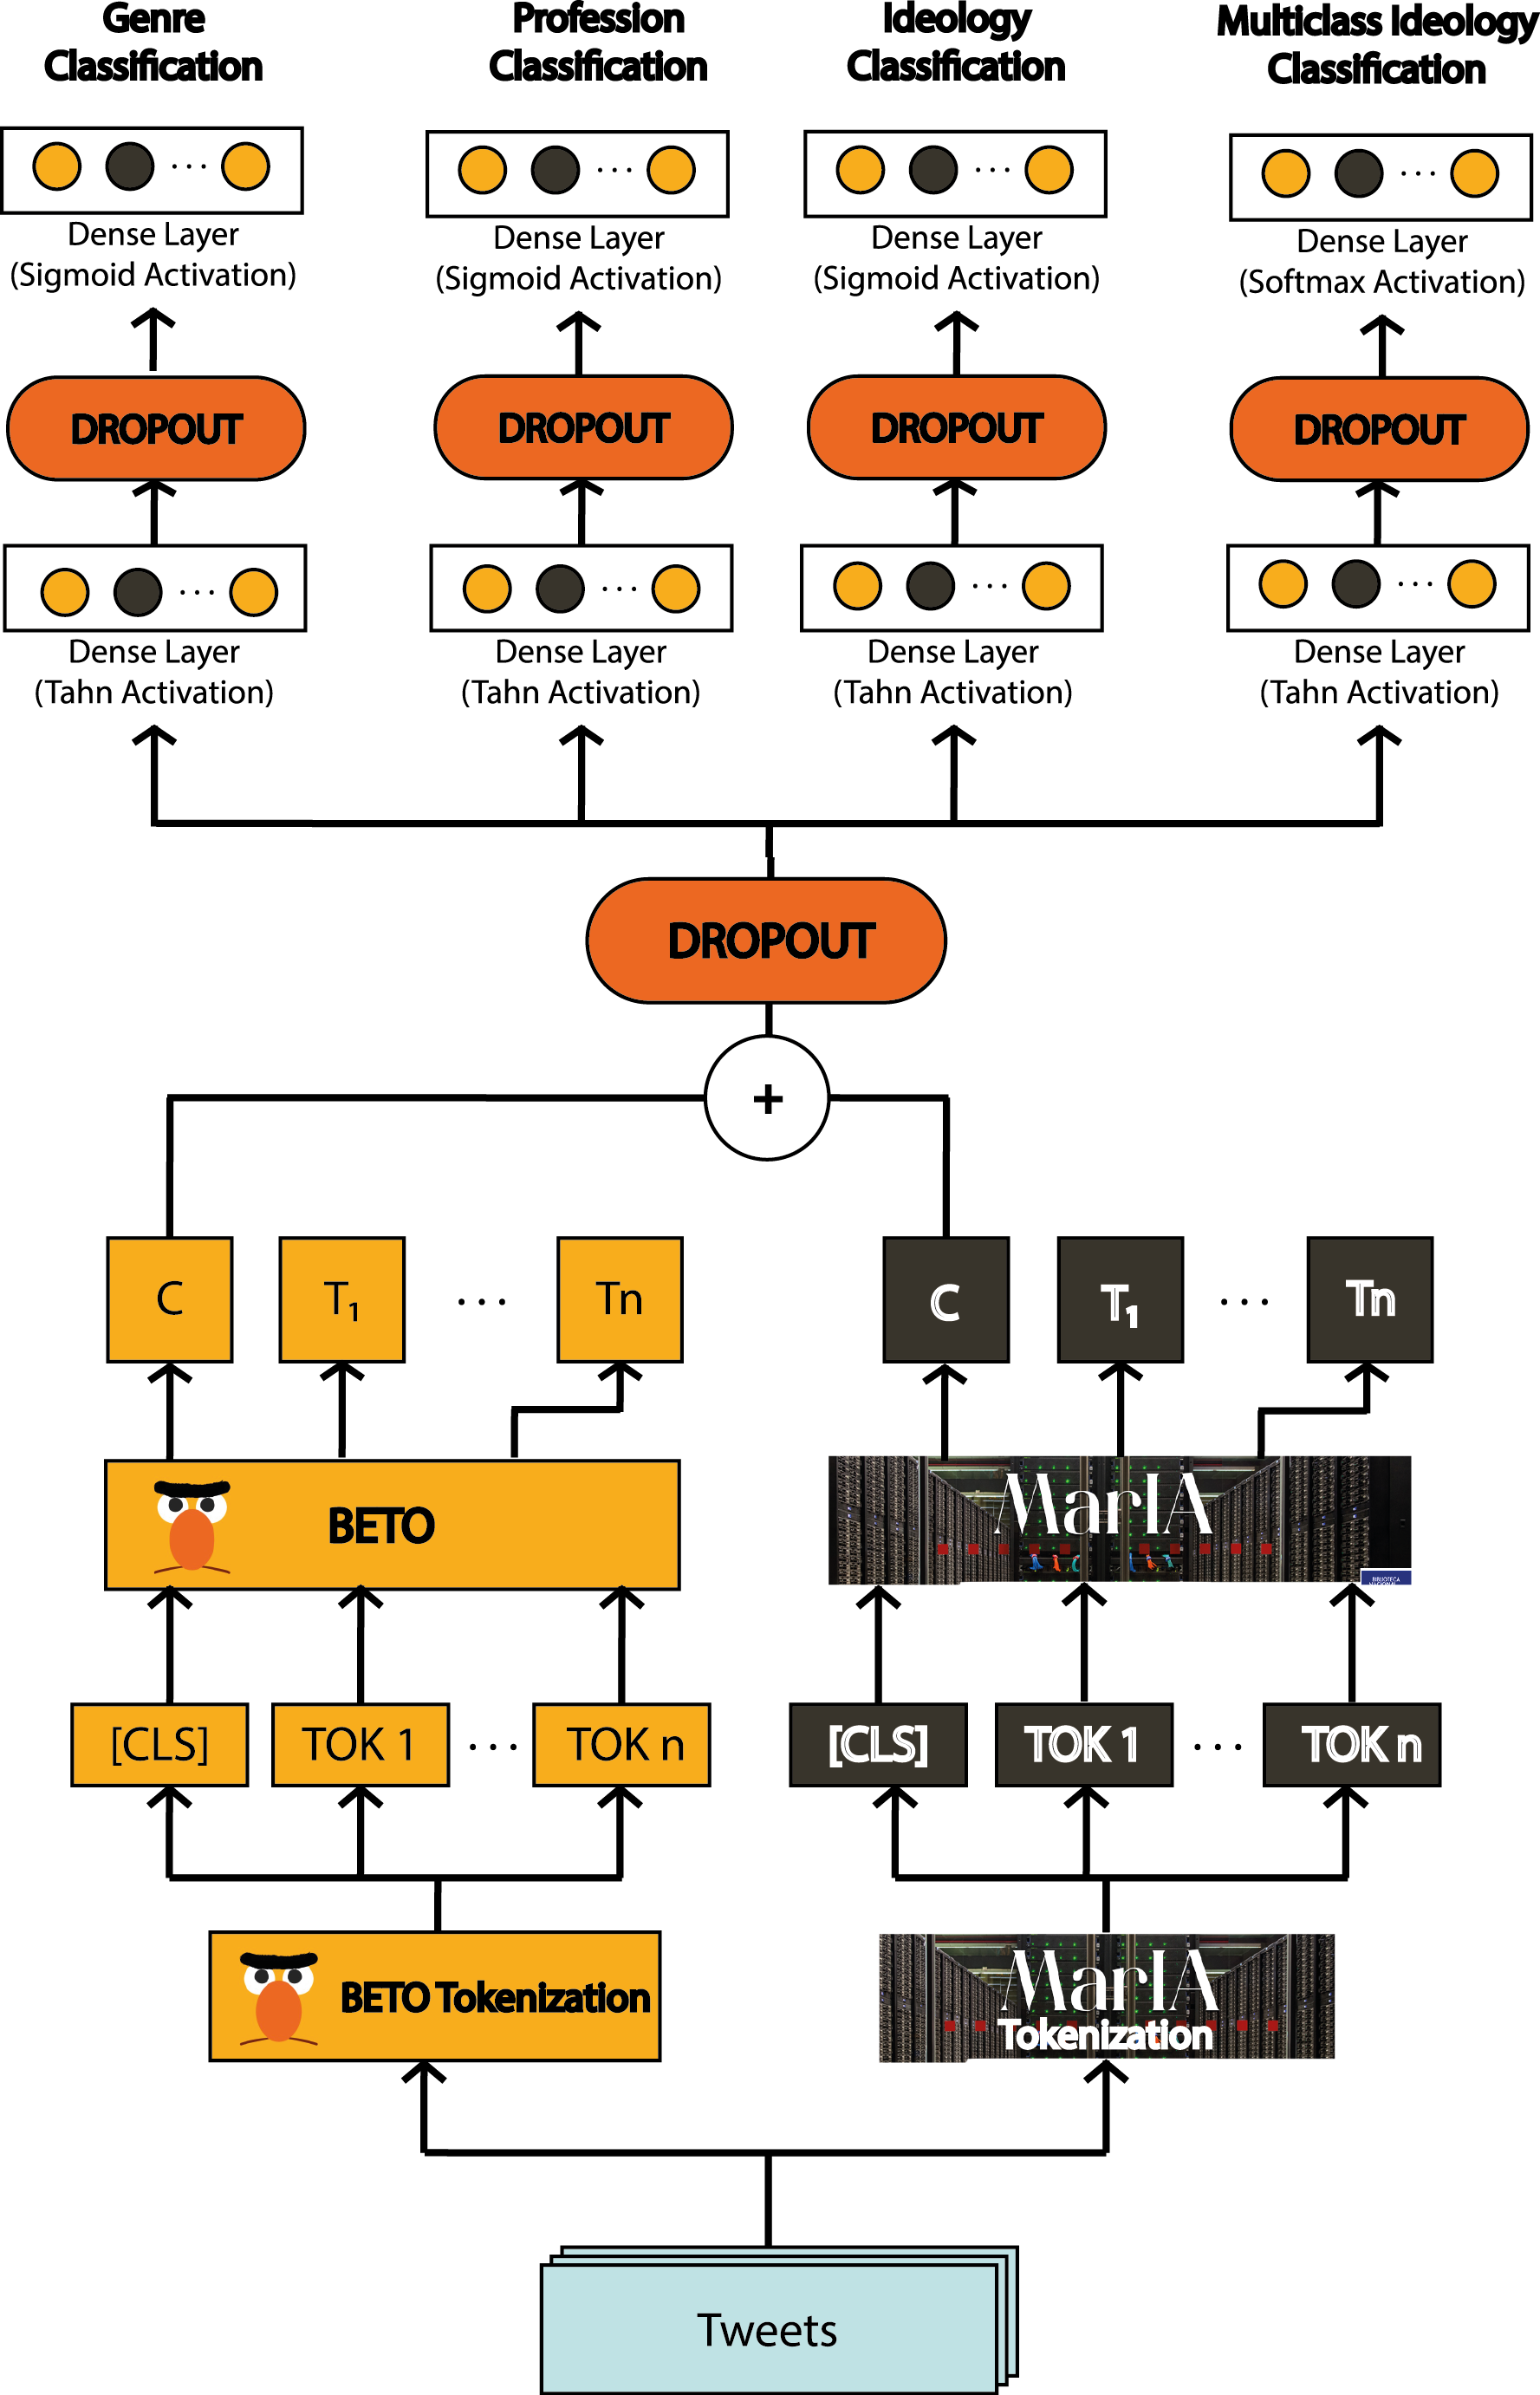
\includegraphics[height=0.8\textwidth]{imaxes/arquitectura_.png}
  \caption{Arquitectura del modelo ganador de la competición de Political Author Profiling del IberLef 2022, utilizado por LosCalis \cite{loscalis22}.}
  \label{fig:arquitectura}
\end{figure}

\subsubsection{Preprocesado}

Por una parte está el preprocesado realizado a la hora de la creación del corpus por los organizadores de la competición. Este consistió en descartar \textit{retweets}, \textit{tweets} donde se parafrasean titulares de periódicos o \textit{tweets} en otros idiomas distintos del español. Además de esto, se anonimizó la colección sustituyendo las menciones a usuarios por el token "@user".\\
Por otro lado, el preprocesado efectuado por LosCalis se limitó a la agrupación de los \textit{tweets} de un mismo autor en bloques de máximo 512 tokens tras la tokenización con BERT y RoBERTa. Esto es así debido a que los modelos basados en BERT no aceptan entradas de mayor tamaño.\\
En nuestro caso, se realizó un preprocesado parecido con la excepción de que se mantuvieron todos los \textit{tweets} de la colección aunque contuvieran fragmentos en otros idiomas o parafrasearan titulares de noticias o blogs. Por un lado, esto se hizo debido a que nuestros \textit{datasets} cuentan con un volumen mucho menor de textos en relación a los corpus de la competición del IberLef, por esa razón decidimos no realizar esa limpieza para mantener un corpus lo más grande posible.

Por otro lado, también se optó por sustituir las \textit{urls} encontradas por el token '<URL>', debido a que en el corpus de la competición no se incluían estas tampoco. Además, se optó por sustituir los emoticonos encontrados en el texto por el token '<EMOTICON>' y los emojis por su descripción sacada de la librería emoji\footnote{\url{https://pypi.org/project/emoji/}}.

\subsubsection{Modelo}
En nuestro caso se replicó el mismo modelo usado por los participantes de la tarea, con las adaptaciones debidas para en las salidas de la red neuronal. En el caso de LosCalis, tenían tres salidas binarias (género, profesión, ideología binaria) y una multiclase (ideología multiclase). En nuestro problema, se tienen únicamente dos salidas: género y edad. En consecuencia se utilizó la arquitectura que se puede ver en la figura \ref{fig:arquitectura_adaptada}. En ella se muestra que se mantienen las mismas capas y funciones de activación que en la arquitectura original con la diferencia de que en vez de cuatro bloques separados de decodificación de las etiquetas, ahora tenemos únicamente dos.

\noindent\begin{figure}[hp!]
  \centering
    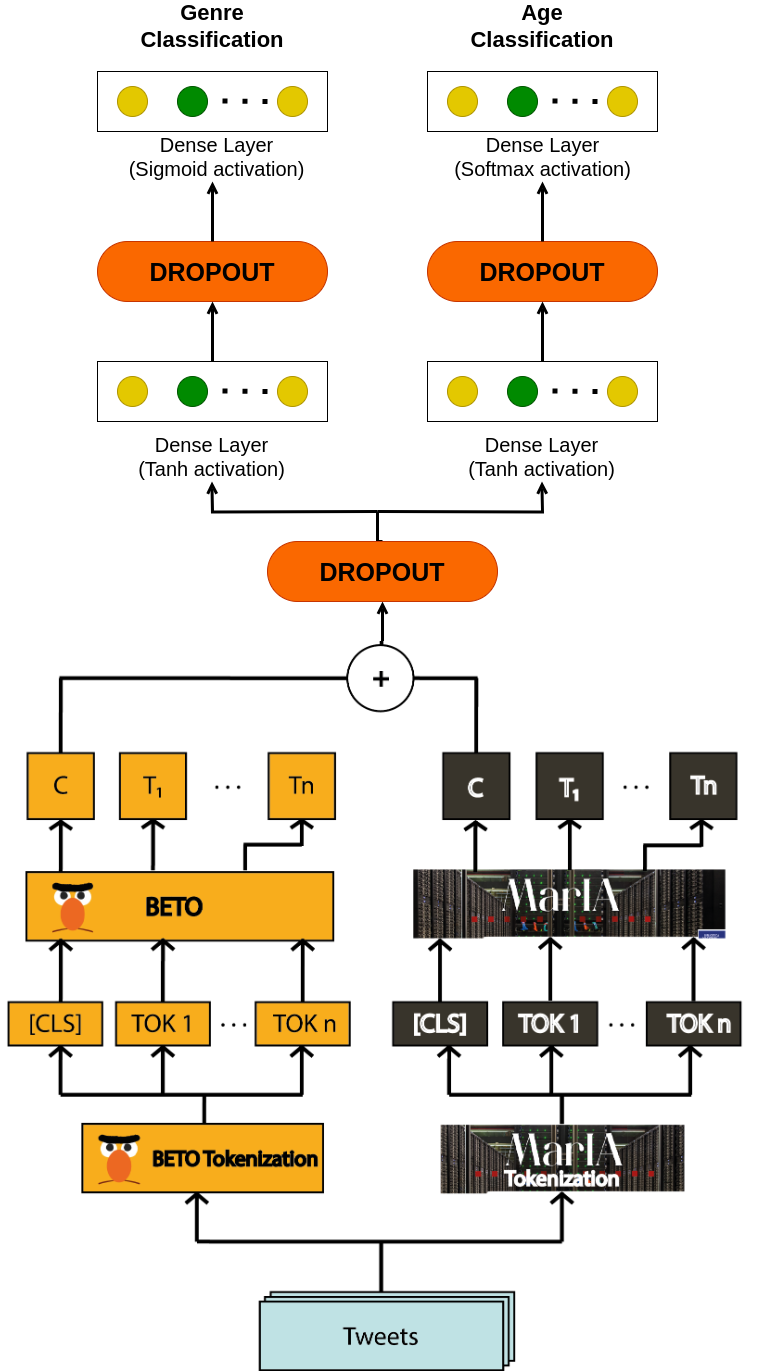
\includegraphics[height=0.8\textwidth]{imaxes/diagrama_arquitectura_profiler.png}
  \caption{Arquitectura basada en transformers adaptada de la aproximación de \cite{loscalis22}.}
  \label{fig:arquitectura_adaptada}
\end{figure}

\subsubsection{Experimentos realizados}
Se realizaron distintas pruebas con los conjuntos de datos expuestos en la sección \ref{sec:datasets}. Para estas se utilizaron la misma configuración de hiper-parámetros propuesta por \cite{loscalis22}, que se puede ver en la tabla \ref{tab:hiperparametros}. 

\begin{table}[hp!]
    \centering
    % \rowcolors{2}{white}{udcgray!25}
    \begin{tabular}{ll}
        \hline
        % \rowcolor{udcpink!25}
        \textbf{Parámetro}  & \textbf{Valor} \\ \hline
        Train batch size    & 64             \\
        Predict batch size  & 8              \\
        Learning rate       & 3e-5           \\
        Training epochs     & 5              \\
        Max sequence lenght & 512            \\
        Dropout             & 0.15           \\
        Optimizer           & Adam           \\
        Dense layer units   & 768            \\ \hline
    \end{tabular}
    \caption{Hiperparámetros utilizados en los experimentos realizados, propuestos por \cite{loscalis22}}
    \label{tab:hiperparametros}
\end{table}
En la tabla \ref{tab:resultados-bert} se pueden ver los experimentos realizados así como los resultados obtenidos en cada uno de ellos en términos de precisión para género y edad.

\begin{table}[hp!]
    \centering
    \rowcolors{2}{white}{udcgray!25}
    \resizebox{\textwidth}{!}{
        \begin{tabular}{|l|l|l|l|}
            \rowcolor{udcpink!25}
            \hline
            \textbf{Entrenamiento} & \textbf{Test} & \textbf{Género} & \textbf{Edad}\\ \hline
            Training 2015     & Test 2015         & 0.8863   & 0.6250\\
            2015 (Train+Test) & Training 2016     & 0.4865   & 0.2703\\
            Training 2016     & 2015 (Train+Test) & 0.4468   & 0.3191\\
            Training 2016     & Test 2016         & 0.4545   & 0.4181\\ \hline
        \end{tabular}
    }
    \caption{Precisión para género y edad en distintos experimentos realizados utilizando el enfoque propuesto por \cite{loscalis22} con las particiones de entrenamiento y test de las competiciones de PAN de 2015 y 2016.}
    \label{tab:resultados-bert}
\end{table}

Lo primero que llama la atención de estos resultados es la diferencia de rendimiento obtenida usando el \textit{dataset} de 2015, a modo de réplica de la competición del PAN \cite{pan:2015}, con el resto de experimentos realizados.

En el primer caso los resultados obtenidos no se alejan demasiado de los conseguidos por el equipo ganador de la misma: 0.9659 y 0.7955, para género y edad respectivamente.

Sin embargo, cuando se trata de aumentar estos datos para obtener mejores resultados, por ejemplo usando el \textit{dataset} completo de 2015 (entrenamiento y test) para entrenar el modelo y se prueban a predecir los autores del corpus de entrenamiento del 2016 se puede ver como los resultados obtenidos empeoran considerablemente, hasta el punto de ser peores que un clasificador aleatorio. Esto se repite al entrenar con la partición de Training de 2016 y testear con la de 2015 completa o con la de Test de 2016 (competición PAN 2016).

Para solventar este problema, lo primero que se probó fue separar una parte del conjunto de entrenamiento para usarlo como conjunto de validación, con la finalidad de observar como se comportaba la función de pérdida o loss\footnote{}, de la red.
\\ La función de pérdida en aprendizaje automático mide la discrepancia entre la clasificación de las predicciones de la red y los datos reales. En las redes neuronales, el objetivo del entrenamiento consiste en la minimización del valor de esta función en cada ciclo mediante del ajuste del valor de los pesos de las conexiones de la red, por medio del algoritmo de retro-propagación del error. Como se explica en \cite{janocha2017loss}, existen diversas alternativas a la hora de escoger una función de pérdida, sin embargo, para problemas de clasificación es bastante común el uso de la entropía cruzada (pérdida logarítmica), por lo cual es la elegida para nuestro algoritmo.

De esta forma viendo la evolución de la función de pérdida durante el entrenamiento, se podría saber si el sistema estaba sobre-entrenado o no. Pues bien, los resultados de esta prueba se pueden ver en la figura \ref{fig:loss}.
\\
 \begin{figure}[hbtp!]
    \centering
    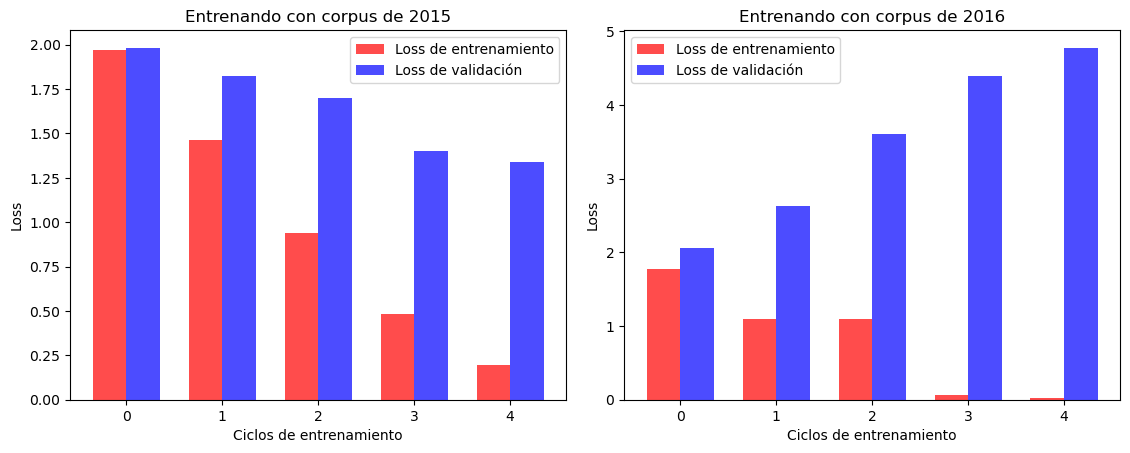
\includegraphics[width=\textwidth]{imaxes/loss.png}
    \caption{Evolución del loss de entrenamiento y validación del modelo propuesto por LosCalis al entrenar con los \textit{datasets} de 2015 y 2016.}
    \label{fig:loss}
\end{figure}
Como se puede ver a la hora de entrenar el modelo con los datos de 2015 el loss del conjunto de validación disminuía al mismo tiempo que el loss del conjunto de entrenamiento; sin embargo, a la hora de entrenar usando el corpus de entrenamiento de 2016 pasaba justo lo contrario, el loss de validación aumentaba cada ciclo mientras el de entrenamiento disminuía (signo de que el modelo se está sobre-ajustando a los datos de entrenamiento y no consigue generalizar).

 Tras descubrir esto, lo primero que se me ocurrió fue investigar un poco los dos conjuntos y compararlos para descubrir si existía alguna diferencia entre ellos. Lo que se descubrió fue que probablemente en el \textit{dataset} de 2015, tanto en el conjunto de entrenamiento como en el de test existían autores repetidos, de modo que el modelo obtenía buenos resultados debido a que el modelo se aprendía el las características textuales de usuarios concretos y no a distinguir la edad o género de una persona aleatoria.
 
 Por otro lado, la diferencia de rendimiento entre el modelo adaptado a nuestro problema y el propuesto por \cite{loscalis22} se especula que se deba probablemente a el mayor tamaño del corpus usado para entrenar en la competición del IberLef (alrededor de 400.000 \textit{tweets} de más de 700 usuarios distintos, frente a 222 usuarios con aproximadamente 800 tweets cada uno) unido a un vocabulario más formal usado por políticos y periodistas españoles junto a unas temáticas mucho más menos variadas, comparado con el vocabulario del usuario promedio de twitter lleno de expresiones de jerga, abreviaturas y disparidad de temáticas tratadas.
 
 Debido a estos malos resultados obtenidos y a la falta de un corpus de mayor tamaño necesario para entrenar un modelo complejo basado en aprendizaje profundo, se decidió orientar el trabajo hacia modelos más sencillos como los expuestos a continuación.



\subsection{Segunda aproximación}
Por otro lado el segundo algoritmo de perfilado probado es el correspondiente a \cite{grivas2015author}. Este obtuvo la tercera posición, en general, en la tarea de author profiling de PAN 2015 (\cite{pan:2015}).
Los \textit{\textbf{datasets}} usados en la competición son los explicados en la subsección \ref{subsec:pan15}.
\subsubsection{Preprocesado}
El preprocesado realizado es distinto dependiendo del tipo de características extraídas. Así los autores de este trabajo separan por un lado características estructurales y características estilométricas.

Las primeras incluyen el numero de menciones, \textit{hashtags} y URLs que contienen los \textit{tweets}. Las segundas, se refieren a la longitud del \textit{tweet} en caracteres y tf-idf n-grams.

Para las estructurales no se realizó ningún preprocesado del texto a parte de concatenar todos los tweets de un autor. Por otro lado, para las estilométricas se eliminaron cualquier tag HTML encontrado, URLs, menciones así como los caracteres '\#' de los \textit{hashtags}.

\subsubsection{Modelo}
Para la clasificación del género, se usó una \gls{svm} con kernel rfb, y se usaron como características únicamente los tf-idf n-grams. En cuanto a la edad, se usó una \gls{svm} con kernel linear a la que se le pasaron como características: tf-idf ngrams, longitud del \textit{tweet}, número de URLs, menciones y \textit{hashtags}. Además, se compensó el desbalanceo de los distintos grupos de edad mediante pesos inversamente proporcionales a la frecuencia de las clases.

\subsubsection{Experimentos y resultados}
En la tabla \ref{tab:aprox2_results} se pueden observar los resultados de los experimentos realizados en esta aproximación. Las métrica elegida tanto para género como edad es la precisión, debido a que es la que se usaba en la competiciones del PAN 2015 y 2016.

\begin{table}[hp!]
    \centering
    \rowcolors{2}{white}{udcgray!25}
    {%
    \setlength{\tabcolsep}{0.6\tabcolsep}
    \begin{tabular}{|l|ll|ll|}
        \hline
        \rowcolor{udcpink!25}
        \textbf{N-gram} & \textbf{Entrenamiento} & \textbf{Test} & \textbf{Género} & \textbf{Edad} \\ \hline
        Carácter [3, 3] & Training 2015 & Test 2015 & 0.9091 & \textbf{0.7159} \\
        Carácter [3, 5 ] & Training 2015 & Test 2015 & \textbf{0.9205} & 0.6932 \\ \hline
        Carácter [3, 3] & Training 2015 & Training 2016 & 0.5766 & 0.3423 \\
        Carácter [3, 3] & Training 2015 & Training 2016 & 0.5856 & 0.3018 \\
        Carácter [3, 3] & 2015 (Train+Test) & Training 2016 & 0.5405 & 0.3468 \\
        Carácter [3, 5] & 2015 (Train+Test) & Training 2016 & 0.5586 & 0.2972 \\ \hline
        Carácter [3, 5] & Training 2016 & 2015 (Train+Test) & 0.5638 & 0.4627 \\ \hline
        Carácter [3, 5] & Training 2016 & Test 2016 & 0.5091 & 0.4545 \\ \hline
        Carácter [3, 3] & Training 2016 & *10-Fold CV & 0.6712 & \textbf{0.5045} \\
        Carácter [3, 5] & Training 2016 & *10-Fold CV & 0.6757 & \textbf{0.5045} \\
        Carácter [5, 8] & Training 2016 & *10-Fold CV & 0.6667 & \textbf{0.5045} \\
        Palabra  [1, 3] & Training 2016 & *10-Fold CV & \textbf{0.6937} & 0.4910 \\ \hline
        Carácter [3, 3] & 2015+2016 (Train) & *10-Fold CV & 0.7024 & 0.6073 \\
        Carácter [3, 5] & 2015+2016 (Train) & *10-Fold CV & \textbf{0.7170} & 0.5707 \\
        Carácter [5, 8] & 2015+2016 (Train) & *10-Fold CV & \textbf{0.7170} & \textbf{0.6195} \\
        Palabra  [1, 3] & 2015+2016 (Train) & *10-Fold CV & 0.6610 & 0.5390 \\
        Palabra  [1, 1] & 2015+2016 (Train) & *10-Fold CV & 0.7122 & 0.5829\\ \hline
        \end{tabular}%
    }
    \caption{Resultados en términos de precisión para género y edad de los experimentos realizados para la aproximación 2 (modelo propuesto por grivas).}
    \label{tab:aprox2_results}
\end{table}
Una vez más sucede que los resultados obtenidos de replicar la competición del PAN 2015, son mucho mejores que el resto de experimentos realizados, lo que afianza la teoría de que en ese \textit{dataset} existen autores repetidos.

Por otro lado, esta aproximación reporta mejores resultados tanto en género como en edad en el resto de experimentos realizados. Por ejemplo al entrenar con el dataset de 2016 y hacer test con 2015 el perfilador ya es ligeramente mejor que un clasificador aleatorio: 56\% y 46\% de precisión para género y edad respectivamente. Lo que refuerza la idea de que en caso de disponer de un corpus de tamaño relativamente pequeño los modelos tradicionales más sencillos son preferibles a los grandes modelos de lenguaje basadose en aprendizaje profundo y transformers que están de moda actualmente.

Los resultados de replicar la competición de PAN 2016 (entrenamiento 2016 y test 2016) muestran como este modelo no generaliza bien a otros géneros a parte de Twitter como son los textos de Blogs, utilizados en el \textit{dataset} de Test de 2016.

Para finalizar, en las últimas filas de la tabla se investigó acerca del tipo de características basadas en n-grams que mejor funcionaban en estos \textit{datasets}. Para ello se utilizó un 10-fold Cross-Validation con el dataset de training de 2016 y el dataset de training de 2016 sumado al de 2015 completo (Training y Test). El cross-validation se utilizó en parte para evitar el sesgo de que pueda haber autores repetidos en los datos del 2015 y porque en 2016 la partición de Test contenía textos de un género distinto (textos de Blogs) que la de entrenamiento. Los resultados que se sacan de estos experimentos son que los n-grams basados en secuencias de 1-3 palabras son las que mayor precisión alcanzan para la predicción de género. Mientras que, los n-grams basados en secuencias de  5-8 caracteres son las que mejores resultados obtienen para edad. No obstante, entre los rangos probados no hay una diferencia significativa de rendimiento en la clasificación.
\subsection{Tercera aproximación}
El último perfilador analizado es el correspondiente al trabajo de \cite{modaresi:2016}. Este fue propuesto para la competición del PAN 2016. En ella los participantes debían realizar un modelo que predijese el género y edad de autores de textos sacados de Blogs\footnote{\url{https://www.blogger.com/about/}} habiendo entrenado el mismo mediante textos sacados de usuarios de Twitter (\ref{sec:datasets}). Por lo tanto, ese algoritmo debe ser lo más independiente del género de escritura posible, lo cual es beneficioso para nuestro problema, ya que entrenamos con textos sacados de una red social como Twitter para predecir usuarios de Reddit.

En esta competición los resultados fueron bastante bajos comparados con las anteriores: el autor de este modelo (\cite{modaresi:2016}), el cual quedó en segunda posición en idioma español, obtuvo 0.6964 y 0.5179 para género y edad respectivamente.

\subsubsection{Preprocesado}
El procesado realizado en este algoritmo, tenía la intención de eliminar la información específica de género presente en los textos. De se usaron distintas operaciones de preprocesado en función de las características extraídas del texto. A continuación se enumeran todas las operaciones de preprocesado que se realizan para el perfilado:
\begin{itemize}
    \item p1: Pasar el texto a minúsculas.
    \item p2: Filtrar cualquier URL encontrada.
    \item p3: Eliminar menciones en las que aparezca un nombre de usuario del tipo '@username'.
    \item p4: Eliminar todos los Hashtags del texto.
    \item p5: Eliminar los retweets encontrados (en teoría no existen en el \textit{dataset}).
    \item p6: Eliminar cualquier carácter no latino encontrado.
    \item p7: Eliminar acentos latinos de palabras, para favorecer la precisión de características basadas en n-grams.
    \item p8: Eliminar caracteres no alfabéticos, como aquellos encontrados en emojis.
    \item p9: Eliminar stop-words basadas en una lista predefinida. 
\end{itemize}
Además de estas operaciones se procedió a la típica operación de concatenar los texto procedentes de un mismo autor para la extracción de características.

\subsubsection{Características extraídas}
En la tabla \ref{tab:preprocesado} se especifican las operaciones que se realizaron para cada tipo de característica extraída. A continuación se explica en que consisten estas:
\begin{table}[hp!]
    \centering
    \rowcolors{2}{white}{udcgray!25}
    \begin{tabular}{|l|l|}
        \rowcolor{udcpink!25}
        \hline
        \textbf{Característica} & \textbf{Operaciones de preprocesado} \\\hline
        Unigrams & p9 ◦ p8 ◦ p7 ◦ p6 ◦ p5 ◦ p4 ◦ p3 ◦ p2 ◦ p1 \\
        Bigrams & p8 ◦ p7 ◦ p6 ◦ p5 ◦ p4 ◦ p3 ◦ p2 ◦ p1 \\
        Promedio de errores de escritura & —— \\
        N-grams de caracteres & p2 ◦ p3 ◦ p4 ◦ p1 \\
        Características de puntuación & —— \\ \hline
    \end{tabular}%
    \caption{Operaciones de preprocesado realizadas según la característica extraída del texto.}
    \label{tab:preprocesado}
\end{table}
\begin{itemize}
    \item \textbf{Unigrams} y \textbf{Bigrams}: consisten en secuencias de n-grams basadas en palabras de longitud uno y dos respectivamente.
    \item \textbf{Promedio de errores de escritura}: se determina un valor relativo para las palabras correctamente escritas y se va sumando, de modo que cuanto mayor sea esta suma en relación a la longitud del texto, menores errores de escritura habrá.
    \item \textbf{N-grams de caracteres}: en concreto se utilizan secuencias de longitud 4, de caracteres con límites, es decir, los caracteres de la secuencia deben pertenecer todos a la misma palabra.
    \item \textbf{Puntuación}: además se mide el número promedio de comas, puntos y marcas de exclamación del texto.
\end{itemize}
Para la predicción de la edad se usaron todas estas características, para el género se omitió la puntuación.

\subsubsection{Modelo}
En este algoritmo, se probó con diferentes técnicas como Gradient Boosting o Random Forests, sin embargo los resultados obtenidos por medio de Regresión Logística fueron superiores. Por ello se empleó este modelo.\\
Se usa la estrategia uno frente a todos para la clasificación multiclase de la edad. Ademñas se establece el hiperparámetro $C=10^{-3}$.
\subsubsection{Experimentos y resultados}
En la tabla \ref{tab:results_aprox3} se muestran los experimentos realizados en esta aproximación. Como en las anteriores la métrica utilizada es la precisión.

\begin{table}[hp!]
    \centering
    \rowcolors{2}{white}{udcgray!25}
    {
    \setlength{\tabcolsep}{0.6\tabcolsep}

    \begin{tabular}{|l|l|ll|ll|}
        \hhline{------}
        \rowcolor{udcpink!25}
          \multicolumn{2}{|c|}{Dataset} & \multicolumn{2}{c|}{Género} & \multicolumn{2}{c|}{Edad} \\ \hline
        \textbf{Entrenamiento} & \textbf{Test} & \textbf{Acc} & \textbf{F1} & \textbf{Acc} & \textbf{F1}\\ \hline
        Training 2015 & Test 2015 & 0.8977 & 0.8977 & 0.5795 & 0.5795 \\
        2015 (Train+Test) & Training 2016 & 0.6368 & 0.6368 & 0.3722 & 0.3722\\
        Training 2016 & 2015 (Train+Test) & 0.6968 & 0.6968 & 0.3830 & 0.3830 \\
        Training 2016 & Test 2016 & 0.5818 & 0.5818 & 0.5090 & 0.5090 \\
        Training 2016 & *10-Fold CV & 0.7657 & 0.7657 & 0.5124 & 0.5124 \\
        2015+2016 (Train) & *10-Fold CV & 0.8173 & 0.8173 & 0.6423 & 0.6423\\ \hline
    \end{tabular}%
    }
    \caption{Resultados en términos de precisión para género y edad de los experimentos realizados para la aproximación 3 (modelo propuesto por modaresi).}
    \label{tab:results_aprox3}
\end{table}

En esta ocasión se puede ver como sigue el patrón de resultados muy buenos para el benchmark de la competición del PAN 2015: género alrededor de 90\% de precisión, y para la edad en este caso los resultados son bastante peores que en con los otros dos modelos.

Sin embargo, esta aproximación mejora a las otras dos en cuanto al perfilado para géneros distintos (entrenamiento y test 2016), donde vemos que el género ya supera el 50\% de precisión y la edad lo alcanza también.

En líneas generales, se puede observar que esta aproximación mejora significativamente a las otras dos en la predicción del género sobre todo, pues consigue una precisión media de 76\% para el 10-fold Cross-Validation del \textit{dataset} de 2016 y llega al 81\% si añadimos el corpus del 2015, frente al 69\% y 71\% de la aproximación 2. En cuanto a la predicción de la edad no obstante, no se aprecia una mejora significativa con respecto a la segunda aproximación.


% \begin{table}[hp!]
%     \centering
%     \rowcolors{2}{white}{udcgray!25}
%     \begin{tabular}{llll}
%         \rowcolor{udcpink!25}
%         \multicolumn{3}{c}{\textbf{PAN 2015}}              \\ \hline
%         Modelo         & Gender          & Age             \\ \hline
%         Aproximación 1 & 0.8863          & 0.6250          \\
%         Aproximación 2 & 0.9091          & 0.7159          \\
%         Aproximación 3 & 0.8977          & 0.5795          \\ \hline
%         Ganador        & \textbf{0.9659} & \textbf{0.7955} 
%     \end{tabular}
%     \caption{}
% \label{tab:my-table}
% \end{table}